\documentclass[a4paper,11pt]{book}

\usepackage[T1]{fontenc}
\usepackage[utf8]{inputenc}
\usepackage[LGR,T1]{fontenc} % notice LGRx instead of LGR
\usepackage{lmodern}
\usepackage[final]{pdfpages} 
\usepackage[top=2cm, bottom=3cm, outer=3cm, inner=4cm, headsep=14pt]{geometry}
\usepackage{textgreek}
\usepackage{csquotes}
\usepackage[french]{babel}
\usepackage{fancyhdr}
\usepackage{xsim}
\usepackage{tasks}
\usepackage[absolute]{textpos}
\usepackage{ascii}
\usepackage{eurosym}
\usepackage{amsthm}
\usepackage{url}
\usepackage{circuitikz}
\usepackage{float}



\theoremstyle{definition}
\newtheorem{exmp}{Example}[section]

\bibliographystyle{abbrv}
\pagestyle{fancy}
\fancyhf{}
\renewcommand{\footrulewidth}{1pt}
\renewcommand{\thesection}{\arabic{section}}

\lhead{Architecture des ordinateurs}
\rhead{Les portes logiques}
\rfoot{Page \thepage}

\begin{document}

\chapter{Les portes logiques}
Dans ce chapitre, nous allons détailler les différentes portes logiques, leur fonctionnement et leurs particularités.

Dans la suite de ce chapitre, nous proposons des tables de vérité avec des 0 et des 1, ce qui est un raccourci pour table de vérité représentée en binaire avec 0 pour F (Faux) et 1 pour V (Vrai). Ces raccourcis qui peuvent sembler peu rigoureux dans un autre contexte sont courants en informatique.

\section{La porte NON (Inverseur)}
La porte logique NON (NOT en anglais) propose la fonction logique suivante:

\[ A \rightarrow \bar{A}\]

\subsection{Symbole}
\begin{circuitikz}[american]
    \draw (0,0) node (myNOT) [not port]{};
\end{circuitikz}

\subsection{Table de vérité}
  \begin{tabular}{|c||c|}
    \hline
         & \\
        $A$ & $\bar{A}$ \\
    \hline 
        0 & 1 \\
        1 & 0 \\
    \hline
  \end{tabular}


\section{La porte OU}
La porte logique OU (OR en anglais) propose la fonction logique suivante:
\[ A, B \rightarrow A+B\]
\subsection{Symbole}
\begin{circuitikz}[american]
    \draw (0,0) node (myOR) [or port]{};
\end{circuitikz}
\subsection{Table de vérité}
  \begin{tabular}{|c|c||c|}
    \hline
         & &\\
        $A$ & $B$ & $A+B$ \\
    \hline 
        0 & 0 & 0 \\
        0 & 1 & 1 \\
        1 & 0 & 1 \\
        1 & 1 & 1 \\
    \hline
  \end{tabular}

\section{La porte ET}
La porte logique ET (AND en anglais) propose la fonction logique suivante:
\[ A, B \rightarrow A\cdot B\]
\subsection{Symbole}
\begin{circuitikz}[american]
    \draw (0,0) node (myAND) [and port]{};
\end{circuitikz}
\subsection{Table de vérité}
  \begin{tabular}{|c|c||c|}
    \hline
         & &\\
        $A$ & $B$ & $A\cdot B$ \\
    \hline 
        0 & 0 & 0 \\
        0 & 1 & 0 \\
        1 & 0 & 0 \\
        1 & 1 & 1 \\
    \hline
  \end{tabular}

\section{La porte OU Exclusif}
La porte logique OU Exclusif (XOR en anglais) propose la fonction logique suivante:
\[ A, B \rightarrow A\oplus B\]
\subsection{Symbole}
\begin{circuitikz}[american]
    \draw (0,0) node (myXOR) [xor port]{};
\end{circuitikz}
\subsection{Table de vérité}
  \begin{tabular}{|c|c||c|}
    \hline
         & &\\
        $A$ & $B$ & $A\oplus B$ \\
    \hline 
        0 & 0 & 0 \\
        0 & 1 & 1 \\
        1 & 0 & 1 \\
        1 & 1 & 0 \\
    \hline
  \end{tabular}

\section{La porte NON-OU}
La porte logique NON-OU (NOR en anglais) propose la fonction logique suivante:
\[ A, B \rightarrow \overline{A+B}\]

Soit l'inverse de la fonction OU.
\subsection{Symbole}
\begin{circuitikz}[american]
    \draw (0,0) node (myNOR) [nor port]{};
\end{circuitikz}
\subsection{Table de vérité}
  \begin{tabular}{|c|c||c|}
    \hline
         & &\\
        $A$ & $B$ & $A+B$ \\
    \hline 
        0 & 0 & 1 \\
        0 & 1 & 0 \\
        1 & 0 & 0 \\
        1 & 1 & 0 \\
    \hline
  \end{tabular}

\section{La porte NON-ET}
La porte logique NON-ET (NAND en anglais) propose la fonction logique suivante:
\[ A, B \rightarrow \overline{A\cdot B}\]

Soit l'inverse de la fonction ET.
\subsection{Symbole}
\begin{circuitikz}[american]
    \draw (0,0) node (myNAND) [nand port]{};
\end{circuitikz}
\subsection{Table de vérité}
  \begin{tabular}{|c|c||c|}
    \hline
         & &\\
        $A$ & $B$ & $\overline{A\cdot B}$ \\
    \hline 
        0 & 0 & 1 \\
        0 & 1 & 1 \\
        1 & 0 & 1 \\
        1 & 1 & 0 \\
    \hline
  \end{tabular}
  
\section{La porte NON-OU exclusif}
La porte logique NON-OU exclusif (XNOR en anglais) propose la fonction logique suivante:
\[ A, B \rightarrow \overline{A\oplus B}\]

Soit l'inverse de la fonction XOR. De plus cette fonction propose un comparateur qui retourne VRAI (1) si les deux entrées sont identiques.
\subsection{Symbole}
\begin{circuitikz}[american]
    \draw (0,0) node (myXNOR) [xnor port]{};
\end{circuitikz}
\subsection{Table de vérité}
  \begin{tabular}{|c|c||c|}
    \hline
         & &\\
        $A$ & $B$ & $\overline{A\oplus B}$ \\
    \hline 
        0 & 0 & 1 \\
        0 & 1 & 0 \\
        1 & 0 & 0 \\
        1 & 1 & 1 \\
    \hline
  \end{tabular}
  
\begin{exercise}
    Les Circuits Intégrés (CI) contiennent souvent plusieurs portes logiques et coûtent moins cher achetés en grande quantité. Il peut donc être intéressant de réaliser des portes logiques en combinant d'autres portes logiques.
    Dans notre exemple nous allons supposer que nous n'avons que des portes NAND à disposition\footnote{Nous aurions par exemple un IC CMOS SN74HC00 de Texas Instrument avec quatre portes NAND à deux entrées chacune. Ce composant coûte moins de 1CHF pièce. On trouve facilement ses caractéristiques sur le site de Texas Instrument ou sur le site d'un marchant de composants électroniques comme DigiKey.} pour réaliser nos circuits et nous souhaitons donc, pour chaque porte de base, proposer un circuit équivalent constitué de portes NAND uniquement.
    \begin{tasks}(3)
        \task NOT
        \task AND
        \task OR
        \task XOR
        \task NOR
        \task XNOR
    \end{tasks}
\end{exercise}

\begin{exercise}
Avec le logiciel \emph{Logisim}, on peut concevoir automatiquement un circuit en donnant sa table de vérité. On peut de plus donner comme contrainte de n'utiliser que des portes NAND, ce qui nous permet d'obtenir facilement le corrigé de l'exercice précédent.
\end{exercise}

\begin{figure}[H]
\centering
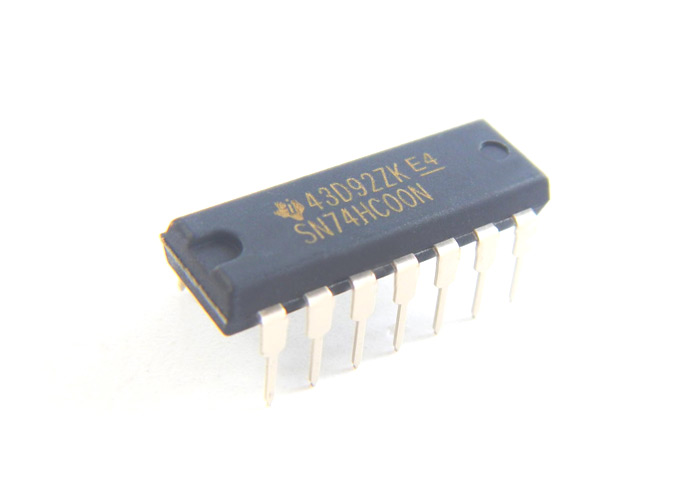
\includegraphics[width=0.5\textwidth]{media/ImplementationGates/SN74HC00-2-Input-NAND-Gate.jpeg}
\caption{SN74HC00 : 4 portes NAND avec deux entrées}
\label{fig:SN74}
\end{figure}

\nocite{fonctionlogique}

%\bibliography{biblio.bib}

\end{document}

